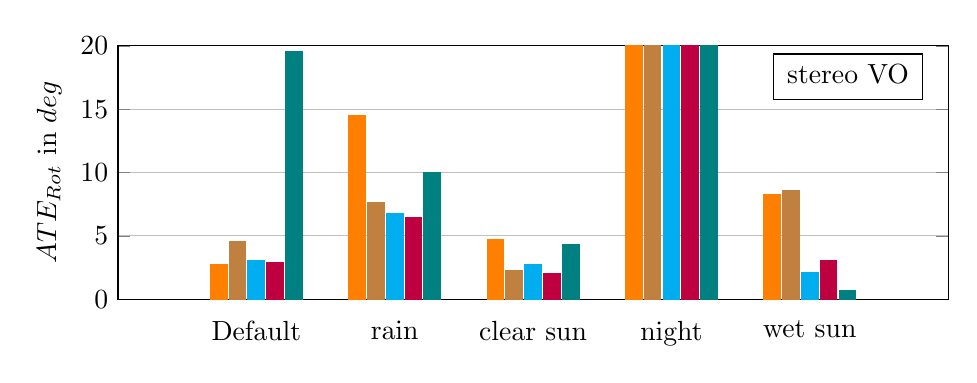
\begin{tikzpicture}
    \begin{axis}[
        width  = \textwidth,
        height = 4.8cm,
        ymax = 20,
        major x tick style = transparent,
        ybar=2*\pgflinewidth,
        bar width=6pt,
        ymajorgrids = true,
        ylabel = {$ATE_{Rot}$ in $deg$},
        % xlabel = {1 Default, 2 hard rain, 3 clear sunset, 4 clear night ,5 wet sunset},
        symbolic x coords={Default, rain, clear sun, night ,wet sun},
        xtick = data,
        scaled y ticks = false,
        enlarge x limits=0.25,
        ymin=0,
        legend pos=north east
    ]
    \addlegendimage{empty legend}
    \addlegendentry{stereo VO}
    \addplot[style={orange,fill=orange,mark=none}]
        coordinates {(Default, 2.73) (rain,14.53) (clear sun, 4.7107) (night ,44.90) (wet sun, 8.24)};
    
    \addplot[style={brown,fill=brown,mark=none}]
        coordinates {(Default, 4.52) (rain,7.65) (clear sun, 2.2452) (night ,20.45) (wet sun, 8.57)};
    
    \addplot[style={cyan,fill=cyan,mark=none}]
        coordinates {(Default, 3.05) (rain,6.74) (clear sun, 2.72) (night ,52.73) (wet sun, 2.11)};
    
    \addplot[style={purple,fill=purple,mark=none}]
        coordinates {(Default, 2.90) (rain,6.43) (clear sun, 1.99) (night , 58.59) (wet sun, 3.06)};
    
    \addplot[style={teal,fill=teal,mark=none}]
        coordinates {(Default, 19.58) (rain,9.99) (clear sun, 4.28) (night , 168.59) (wet sun, 0.672)};
    \end{axis}
  \end{tikzpicture}